\section{Design}
The main design components are: (1) Introspection, (2) Provenance, (3) Data Analysis and (4) Visualization. 
Figure~\ref{designfig:1}(a) shows the interaction among the main components. Figure~\ref{designfig:1}(b) shows the main components of Chimbuko and their interactions.

\begin{figure}[th!]
 \centering
  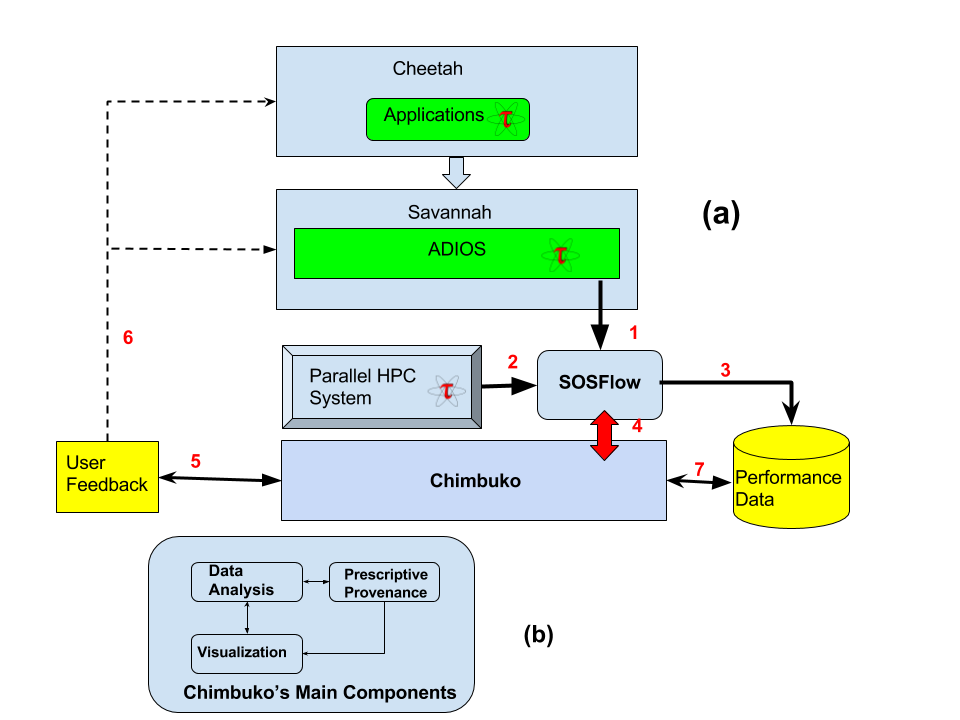
\includegraphics[width=0.65\textwidth]{Figs/Online_Chimbuko}
 \caption{(a) Introspection (b) Chimbuko's main components.}
\label{designfig:1}     
 \end{figure}

\begin{itemize}
\item {\bf{Arrow-1:}} TAU plugin extracts information from application and ADIOS for SOSFlow. 
\item {\bf{Arrow-2:}} TAU plugin extracts system information for SOSFlow.
\item {\bf{Arrow-3:}} SOSFlow stores performance information in performance database.
\item{\bf{ Arrow-4:}} SOSFlow and Chimbuko interaction.
\item {\bf{Arrow-5:}} Feedback module and Chimbuko interaction.
\item {\bf{Arrow-6:}} Feedback to Cheetah and Savannah frameworks.
\item {\bf{Arrow-7:}} Interaction between Chimbuko and performance database.
\end{itemize}

The following performance features will be collected:
\begin{enumerate}
\item For each component in a workflow:
\begin{enumerate}
\item start and end timestamp
\item call stack
\item memory allocation
\item I/O in network or disk
\item total communication time
\item effective communication time
\item effective computation time
\item idle time
\item number of synchronization points/barriers
\item communication size
\item communication between functions
\item communication between nodes
\end{enumerate}
\item For each workflow:
\begin{enumerate}
\item number of components
\item amount of communication for each pair of components
\item effective communication for each pair of components
\item communication size for each pair of components
\item aggregated number of communication calls 
\item aggregated communication execution time
\end{enumerate}
\end{enumerate}
The metadata that needs to be extracted for will vary depending on the application and the node architecture where the application components are run.
For visualization, we will also require the outlier results from the analysis module in terms of the array of call ID, MPI execution ID, or workflow ID.  
We will prioritize detailed communication, understood as MPI communication, followed by I/O.  The choice of communication as a priority for data extraction is motivated by its demonstrated impact on performance for applications such as NWChem and LAMMPS. 

The performance data in Figure~\ref{designfig:1}(a) is collected by TAU and SOSFlow infrastructure based on the information filtered by the prescriptive provenance module of Chimbuko. The data is temporary and will be flushed periodically to make room for the new data.

\subsection{Introspection (TAU + SOSFlow)}
A performance monitoring prototype will be created to enable online access to performance data. This
will consists of two parts:
\begin{enumerate}
\item Extensible Monitoring Plugin Support: TAU will be extended to provide a plugin framework where an event stream will be exported by each MPI rank. An analysis plugin will subscribe to events such as initialization/finalization, metadata values, interval event timers, and counters.  The current hardwired SOS integration will be converted to a plugin. The SOS client plugin will monitor the data stream at runtime and provide aggregation/filtering/reduction utilities.  It will also provide a feedback path to TAU in order to increase/decrease resolution of measurement (sampling rate, callpath depth, hardware counters, etc.) if/when that capability is added to TAU.
\item Online Monitoring Access: Profile, event trace, and metadata events will be provided to the analysis through SOS~\cite{Chad}. In a coupled application/workflow scenario, SOS will regularly/periodically aggregate TAU data over the SOSFlow infrastructure.  This data will be extracted from SOS through an SOS analysis extension that will output the aggregated event stream as ADIOS streaming output.  The SOS extraction client will have the ability to filter data from one or more specific nodes, rather than just an aggregated data stream.  The ADIOS stream will be used by the trace analysis tools and anomaly detection methods.
\end{enumerate}

\subsection{Prescriptive Provenance}
\label{subsection:features}
We will extract, aggregate, and store provenance relevant to online performance analysis and co-design studies with the TAU/SOSFlow plugin and make this information available while the simulation is running.  As provenance can be very verbose and persisting provenance for an entire run is impractical, we will persist detailed provenance {\em only} for the anomaly events or events of interest detected by online performance analysis.  Ultimately, provenance is to be persisted in SOSFlow for a moving window prior to and posterior to an event with the additional capability to increase or decrease the verbosity of provenance (size and granularity of the moving window) selected for storage around the event.  In addition, static information describing the system, runtime configuration, and  workflow or application metadata similar to what is already extracted for offline analysis will be persisted at the on start and end of the run (static information).  This prescriptive provenance,  provenance selection and use prescribed by the results of performance data analysis, is an end product of the analysis after training sets have been built.
Specifications of the moving window of provenance prior to an outlier event will be studied for tradeoffs.  For instance, we will study if this window is defined in terms of execution time or the number of time steps.  Constraints on size and tradeoffs in the amount of details needed will be balanced with usefulness to a scientific code developer.
This prescriptive provenance approach will help reduce the information passed to the data analysis and performance visualization components.

Figure~\ref{designfig:2} explains prescriptive provenance. Suppose we detect an abnormal behavior in performance for a communication intensive workflow component. The event starts at timestamp T2 and ends at timestamp T3. To analyze this event, we need all the communication information within a certain time window at the start of the event and at the end of the event. In Figure~\ref{designfig:2}, ${\bf{X}}$ shows the time window at the start of the event till timestamp T1. The software, hardware, and system information within this time window will be correlated with the communication patterns and performance behavior of the workflow when the event occurred.

\begin{figure}[th!]
 \centering
  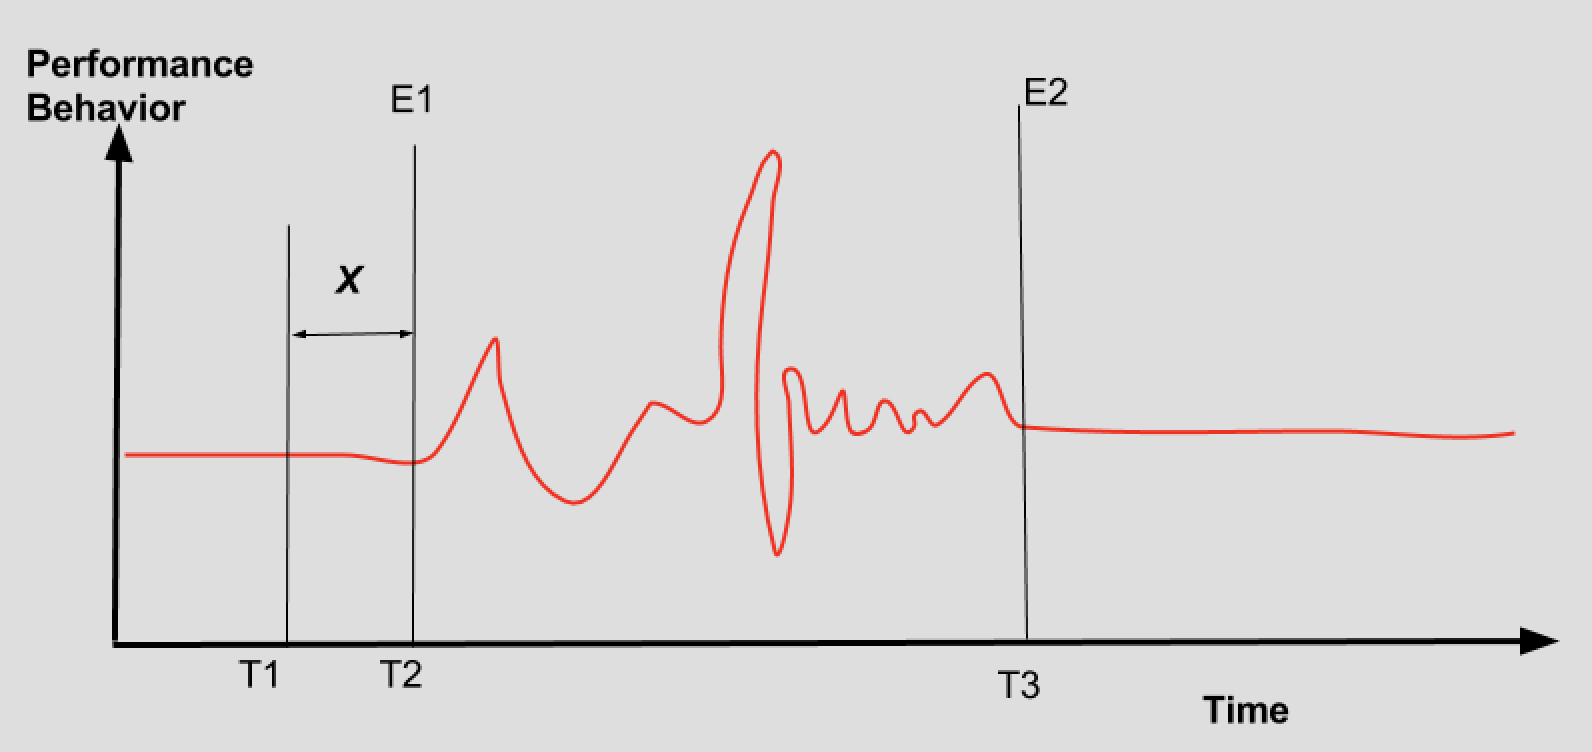
\includegraphics[width=0.5\textwidth]{Figs/Provenance}
 \caption{(a) Prescriptive Provenance.}
\label{designfig:2}     
 \end{figure}

\subsection{Data Analysis}
Last year, we prototyped offline performance anomaly detection by using a Local Outlier Factor (LOF) algorithm. This year we will implement online data analysis by designing and evaluate online anomaly detection algorithms using the features collected by SOSFlow.  The online data analysis could be implemented as two styles: (1) consumer-producer where SOSFlow will be the performance profile/trace stream producer and our online analysis will be the consumer implemented as its client; or (2) via a performance analysis plug-in within SOSFlow to obtain the performance data stream locally.

\subsection{Performance Visualization}
Last year, we developed off-line performance visualization focusing on an ``overview first, details on demand'' scheme. To enable real-time data consumption, analysis before visualization is required.  Therefore, this year, we will provide online performance visualization coupled with performance analysis.  
To establish the connection between the analysis module, SOSFlow, and the user, the visualization module will provide (1) a user exploration interface to visualize, monitor and interact with the analysis results and performance data; and (2) a back end communication channel to the analysis module and streaming data from SOSFlow.   In particular,
we will provide:
\begin{itemize}
%\item A set of visual analytics modules to convey analysis results and provide interaction.
%\item Methods to communicate with the data analysis module and SOSFlow. Two styles are considered: (1) passive mode, where SOSFlow or the analysis module is a server that sends update data to the visualization module as its client; and (2) active mode, where the user queries the detailed information from SOSFlow or the analysis module. 
%\item Methods to maintain a local database collecting only the details of the outliers and other necessary information for users to query workflow details.
\item A set of visual analytics modules to convey analysis results (outliers) and provide interaction in different levels of details.
\item Methods to communicate with the data analysis module and SOSFlow.
\item Methods to communicate with the performance database collecting only the details of the outliers and other necessary information for users to query workflow details.
\end{itemize}

